\subsection{Numerical solution with McCormack's scheme}
We will now present the numerical solution of the shallow water equations using McCormack's scheme and compare it with the one obtained with Lax-Wendroff. The code can be found at the end of the report.

Figures \ref{mc01} and \ref{mc02} present the solution for two different values of the ratio $\frac{\Delta t}{\Delta x}$. For both those plots, the number of point in the x-direction is $N=100$.

\begin{figure}
\begin{center}
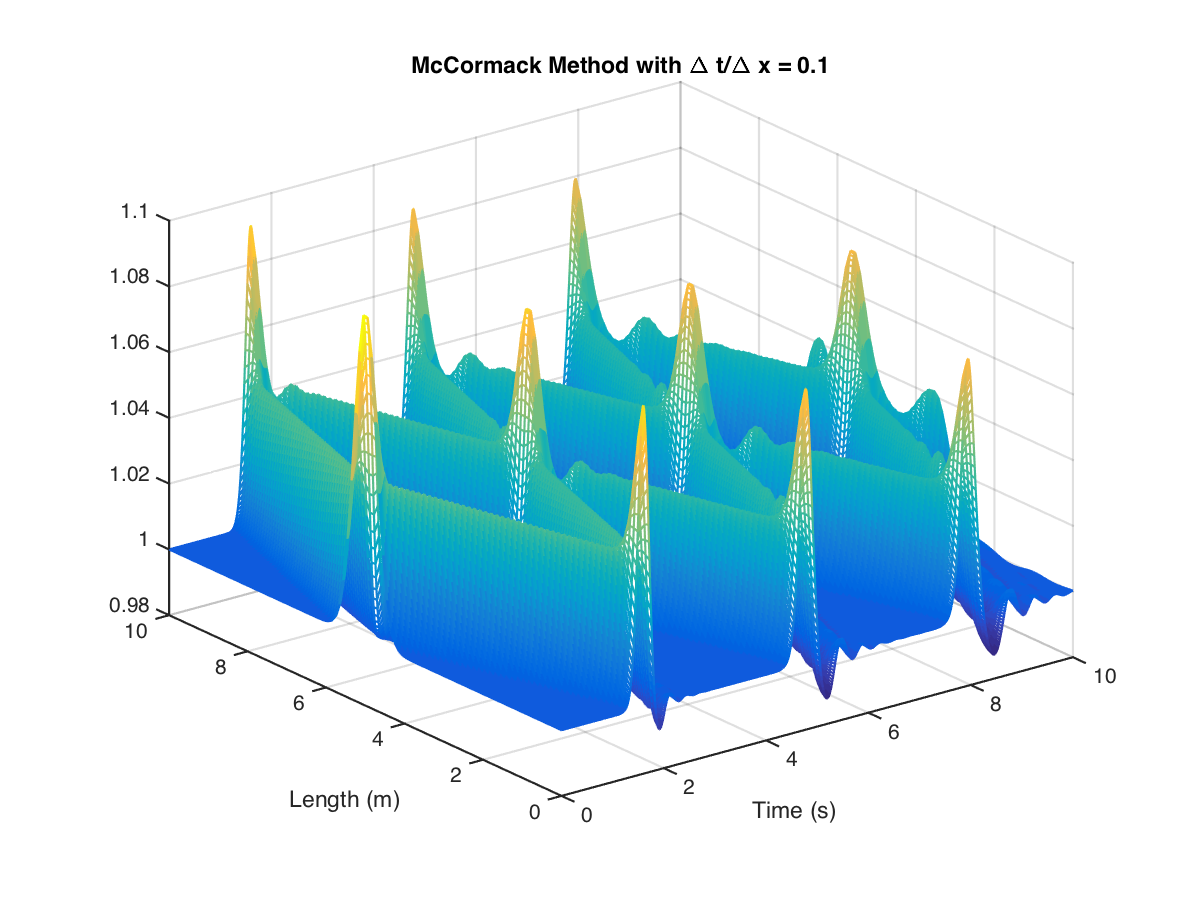
\includegraphics[scale=0.6]{mccormack01.eps}
\caption{Solution for $\frac{\Delta t}{\Delta x}= 0.1$ with McCormack's scheme}
\label{mc01}
\end{center}
\end{figure}

\begin{figure}
\begin{center}
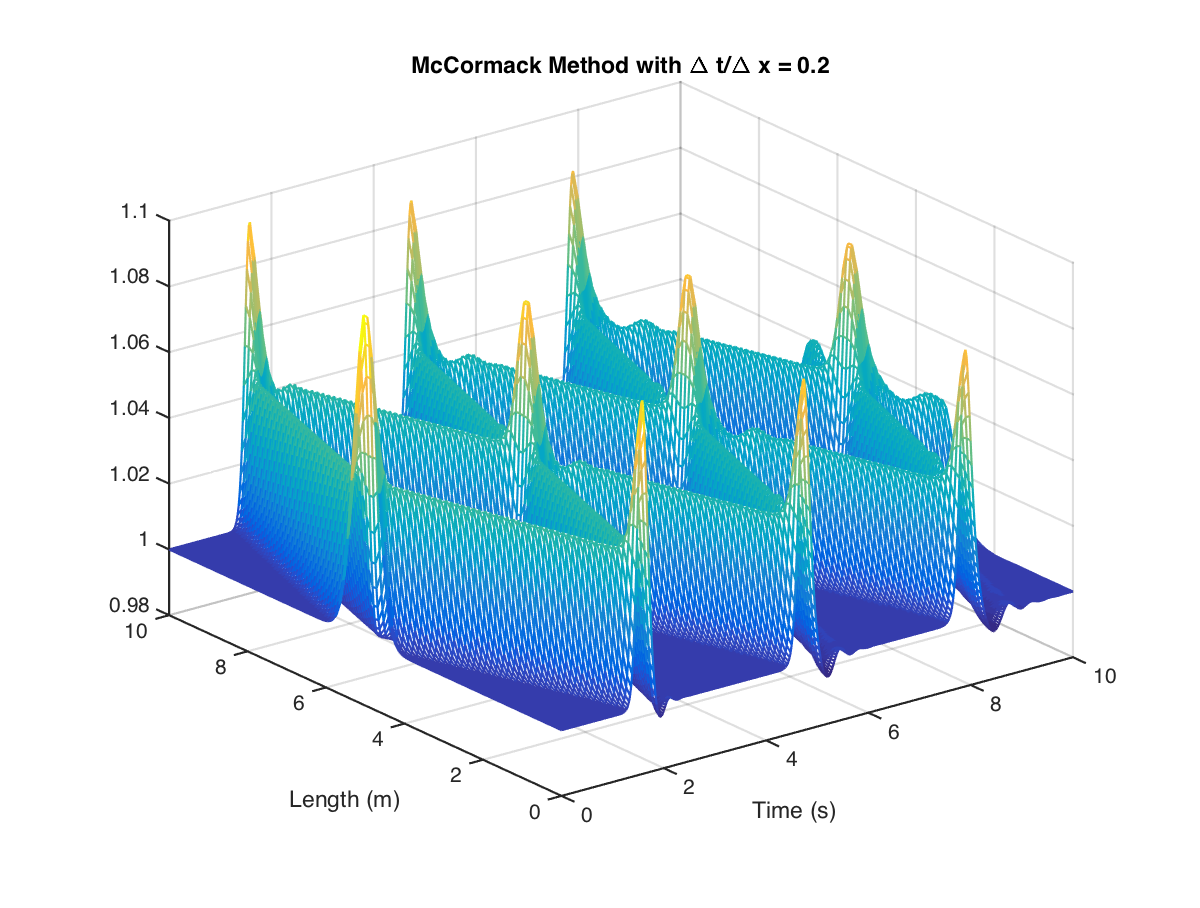
\includegraphics[scale=0.6]{mccormack02.eps}
\caption{Solution for $\frac{\Delta t}{\Delta x}= 0.2$ with McCormack's scheme}
\label{mc02}
\end{center}
\end{figure}

There are several remarks to make. We can first see dispersion errors at the boundary and more generally where the gradients are steep. We can also see that those dispersion errors tend to increase with time. This is particularly visible when the ratio is equal to 0.1. We can also see that the dispersion at the boundary increases when the ratio gets smaller.

To better understand the effects of discretization, we also have figure \ref{mc200}, where the ratio is also equal to 0.2 but with now $N=200$, i.e. the spatial grid has been refined. 
\begin{figure}
\begin{center}
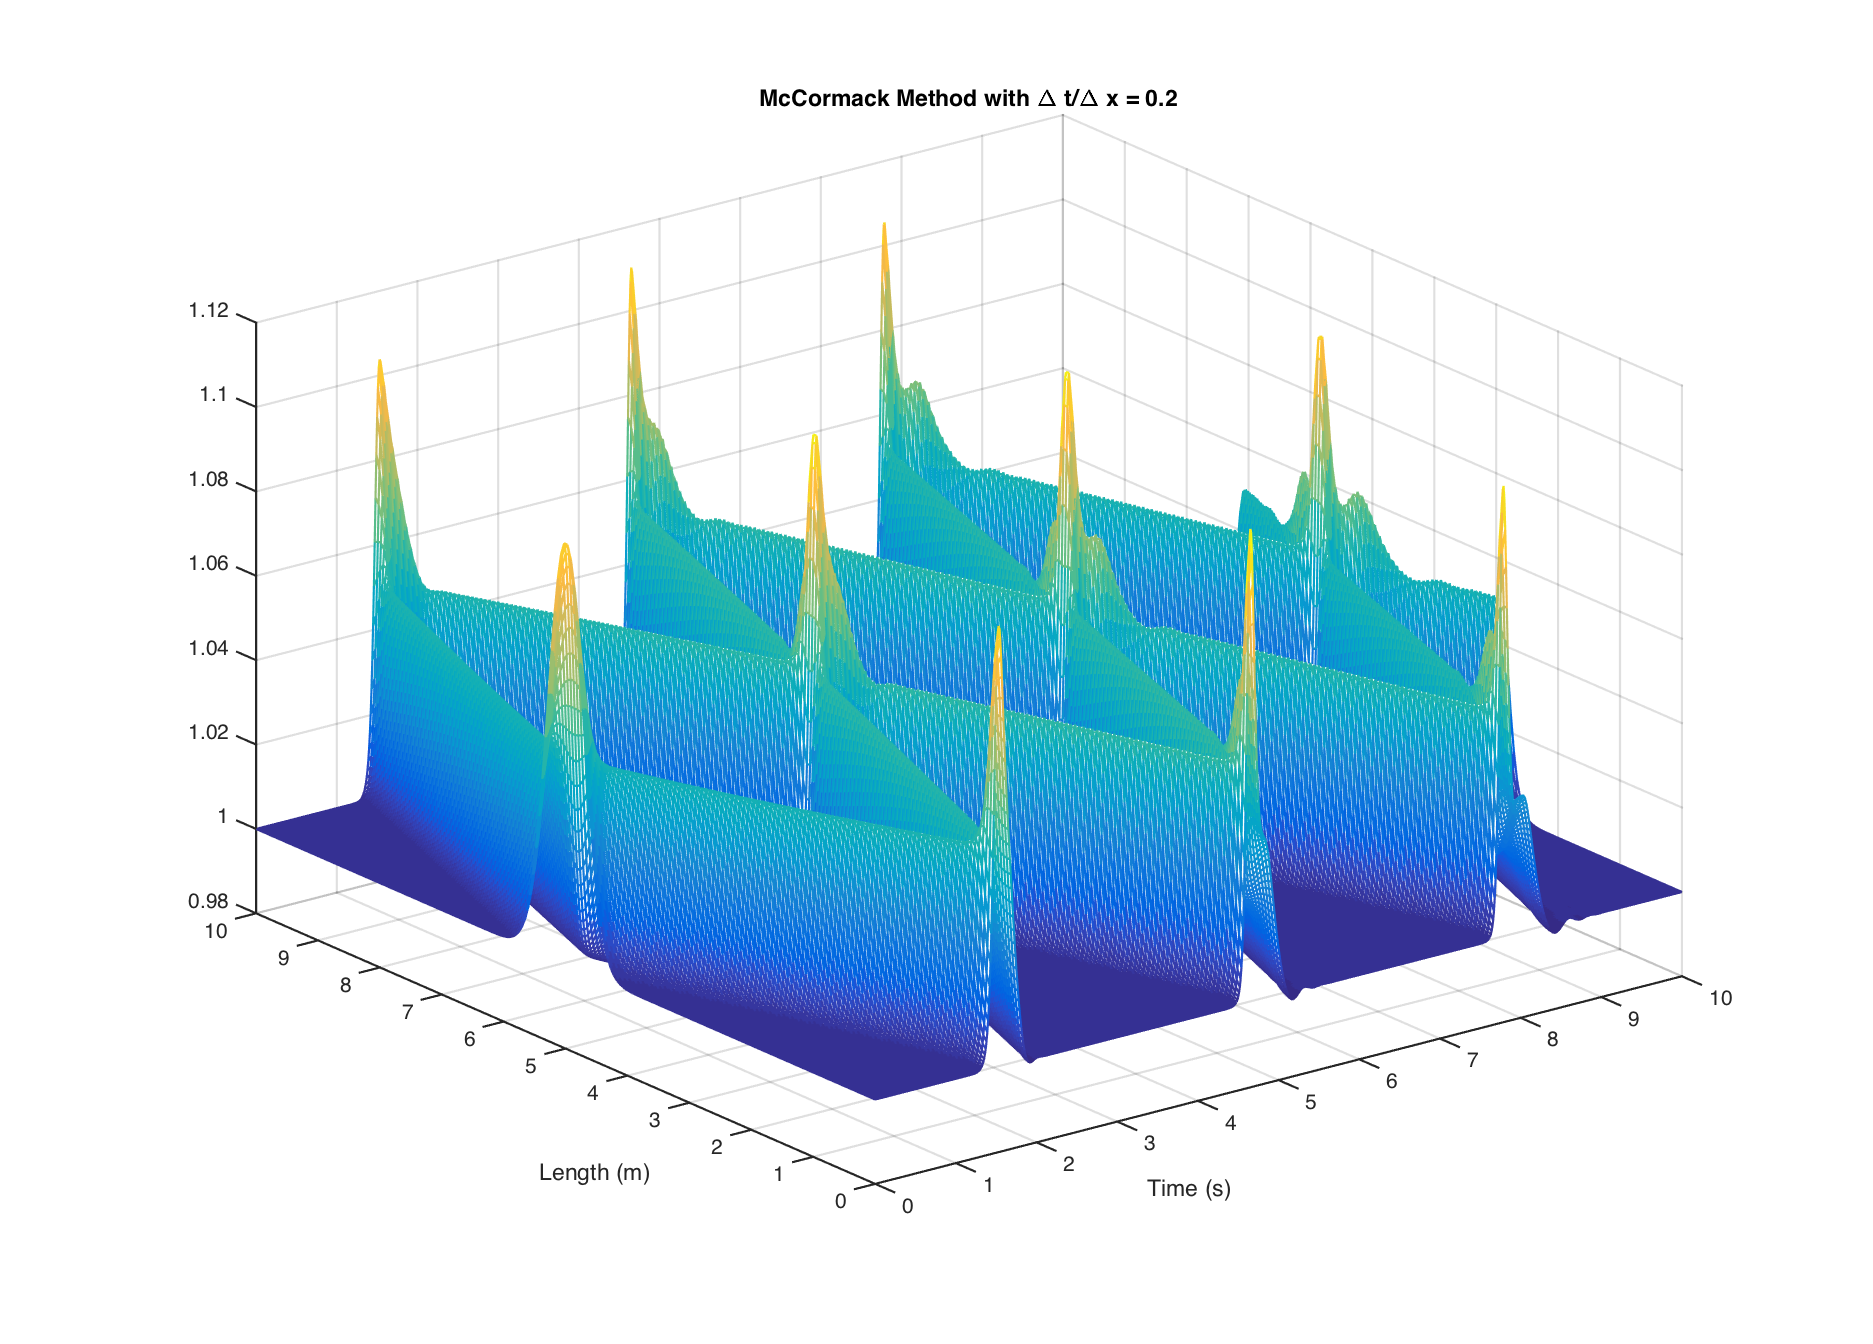
\includegraphics[scale=0.5]{mccormack02200.eps}
\caption{Solution for $\frac{\Delta t}{\Delta x}= 0.2, N=200$ with McCormack's scheme}
\label{mc200}
\end{center}
\end{figure}

Here, we can see that we have smaller dispersion errors at the boundary. However, this is not true around the peaks. There, the dispersion errors look the same or even a bit bigger.

Finally, it is interesting to compare the two methods. With Lax-Wendroff we did not have any dispersion errors as we have with McCormack. However, Lax-Wendroff dissipation errors and the smaller the ratio $\frac{\Delta t}{\Delta x}$ is, the bigger the dampening of the wave we can observe. This does not happen with McCormack, we have no dampening whatever the ratio. Our last remark will be that with both method, the numerical solution is unstable when the ration is larger than 0.3.

